%!TEX encoding = UTF-8 Unicode
%!TEX program = xelatex

\documentclass[bachelor]{ustcthesis}
% bachelor|master|doctor [professional] [english] [pdf] [authoryear|numebers]
\usepackage{ustcextra}
\graphicspath{{figures/}}

\title{基于贝叶斯推断的反垃圾邮件系统}
\author{樊 \em 华}
\school{继续教育学院}
\level{本科}
\form{业余}
\age{3年}
\site{上海理工大学}
\major{计算机软件}
\num{16142233031}
\supervisor{朱明}
%\cosupervisor{钱学森\ 教授}
\date{2018年5月11日}    % 注释掉则为今日
% \date{二〇一七年五月一日}    % 注释掉则为今日
% \professionaltype{专业学位类型}
% \secrettext{机密\quad 小于等于20年}    % 内部|秘密|机密,注释本行则不保密

% \entitle{An Example of USTC Thesis Template for Bachelor, Master and Doctor}
% \enauthor{Zeping Li}
% \enmajor{Mathematics and Applied Mathematics}
% \ensupervisor{Prof. Luogeng Hua}
% \encosupervisor{Prof. Xueshen Qian}
% \endate{May 1, 2017}    % today if commented
% \enprofessionaltype{Professional degree type}
% \ensecrettext{Confidential\quad Less than or equal to 20 years}
% Internal|Secret|Confidential

\begin{document}

\maketitle

% 本科论文:
%   frontmatter: 致谢、目录、中文摘要、英文摘要
%   mainmatter: 正文章节、参考文献
%   appendix: 附录
%
% 硕博论文:
%   frontmatter: 中文摘要、英文摘要、目录、符号说明
%   mainmatter: 正文、参考文献
%   appendix: 附录
%   backmatter: 致谢、发表论文

\frontmatter
%!TEX root =  ../main.tex
\pagestyle{empty}
\begin{abstract}
  电子邮件系统目前互联网上最普及的应用之一。然而,电子邮件在给人们提供便捷通信手段的同时,也遭到了一些人为的滥用。当今垃圾邮件问题已经愈演愈烈,对互联网造成了很大危害。利用技术方法来阻挡垃圾邮件,是目前为止对付垃圾邮件问题最有效的手段。各种过滤技术中,贝叶斯过滤技术,借鉴了在文本挖掘问题中获得成功的机器学习算法,是目前研究较多的一种过滤技术。贝叶斯过滤方法在分类的效果上以及在不需要太多人工干预上都有很大优势,因此逐渐被广泛接受。
  
    我们分析了目前的垃圾邮件内容过滤技术,认识到垃圾邮件过滤技术与普通的文本分类和挖掘问题存在着很多不同。我们总结和分析了目前基于贝叶斯垃圾邮件过滤技术的现状,包括文本表  示、特征选择、分类算法、评价体系,以及垃圾邮件过滤领域中常用的公共语料库,对基于贝叶斯的过滤方法提出了一系列改进。论文的具体内容包括:  
     
    (1)对朴素贝叶斯算法进行了详细的研究,并且提出了三个方面的改进思路。在文本表示方面,提出采用指纹特征的表示方法;在特征选择方面,提出了基于类条件分布的特征选择;第三个方面,根据学习的不断深入性,提出了阈值动态调整算法。基于这些改进,实现了改进的朴素贝叶斯过滤器。 
    
    (2)分析邮件结构特点,从邮件结构不同于普通文本出发,提出集成加权模型,以充分利用邮件的结构信息。基于集成加权模型对邮件头和邮件正文分别建立模型,最后通过加权方法集成二者结果,对垃圾邮件进行过滤。
      
    (3)研究了最小风险贝叶斯和主动学习贝叶斯两种贝叶斯的扩展模型。最小风险贝叶斯能够减少正常邮件判为垃圾邮件的风险,而主动学习贝叶斯主动训练样本集,能够降低样本顺序对过滤精度的影响。根据实验结果对比,得到两种扩展模型的最佳应用条件,并提出了改进后的邮件过滤算法。  综合以上改进和扩展而设计的贝叶斯过滤器在最新的标准数据集上的测试结果表明,与经典的贝叶斯过滤器Bogo相比,过滤效果有较大的提高。 
  \keywords{集成加权贝叶斯;最小风险贝叶斯;主动学习贝叶斯;特征选择;阈值调整}
\end{abstract}

\begin{enabstract}
  Electronic mail (e-mail) is a big success of Internet; it is becoming one of the fastest  and most economical ways of communication available. At the same time,the growing problem of junk mail (also refered to as “spam”) has generated a need for e-mail filtering. There have been a lot of methods to beat spam, and the approach of using automated text categorization and information filtering to filter spam is become a most efficient one. We analyzed the current technology of content-based spam filtering, and found lots of differences between the traditional text categorization Problem and the one of spam filtering. Depend on this analysis, develop some methods to improve the performance of the spam filtering algorithm.
  
  The contents of this article are as following:
  
  (1) A summary about the state of the content-based spam filtering. We investigating anti-spam problem from the text categorization perspective, introducing the approaches of feature selection, classifiers and e-mail corpus in this task. 
  
   (2) We study the bayes algorithm in details and propose the improvings in four aspects.The first aspect is the showing of text.We proposes a new method which is fingerprint feature. The second aspect is feature selecting. We propose a new method which is class condition distribute. The e-mail corpus and text corpus are very different in structure. We analyzed the structure of email, and purposed a email header and email body integrated model. In the fourth aspect, we propose threshold adjusting algorithm. In the end ,we combine four aspects, and realize the improving bayes percolator. 
   
    (3)  From the shortcomings of ordinary  bayes,Bayes proposed minimum risk  Bayes model and initiative studying  Bayes model. Minimum risk Bayes model reduced the risk to judge the normal mail as spam email And the initiative  studying  Bayes model can reduce  the impact of the order of corpus in the email filtering accuracy. 

  \enkeywords{Minimum risk bayes ; Active learning bayes ; Integration weighted bayes ; Feature selection ;   Threshold adjustment}
\end{enabstract}

\tableofcontents
% \listoffigures
% \listoftables
% \listofalgorithms
% \input{chapters/0.notation}

\mainmatter
\chapter{绪论}

\section{引言}

\subsection{课题研究背景}
Internet的迅速发展,人与人的交往更加方便,电子邮件以其快捷低廉的特性逐渐成为人们信息交互的重要工具。人们用它来交流思想,传输文件,发表意见等,逐渐成为日常生活中不可缺少的通信工具。但是电子邮件在其给人们带来极大便利的同时也带来了一些负面影响,那就是我们每天收到的邮件有很大一部分是不请自来的。它们有些是商业广告,有些是政治宣传,有些是色情广告,还有一些甚至是病毒,这就是我们俗称的垃圾邮件。

根据美国nucleus  research 公司公布的数据,全球每天大约有140亿封垃圾邮件在网上传播,相当于地球上每个人每天都要收到两封以上的垃圾邮件。  

垃圾邮件给网民造成的经济损失是相当惊人的:据统计仅下载它们所花费的上网费和电话费用等费用,每年就会花掉全球网民94美元。作为垃圾邮件的发送方,价格是及其低廉的,通常是通过各种方式群发。而对于电子邮件服务提供商和用户来说,垃圾邮件却给他们带来了很大的危害和损失,而且如色情,电脑病毒,以及荷重欺诈信等造成的损失更是造成难以评估。
\subsection{贝叶斯研究简介}
贝叶斯的论文“关于几率性问题求解的理论”奠定了贝叶斯学派的基础。而后著名数学家laplace用贝叶斯理论导出的”相继律”使得贝叶斯理论受到人们的关注。但是由于当时贝叶斯方法在理论和实际的应用中还存在很多不完善的地方,因而在十九世纪并未被人接受。八十年代以后,人工智能的发展尤其是机器学习,数据挖掘等兴起,为贝叶斯理论的发展和应用提供了更为广阔的空间。 

 尽管对于贝叶斯学派哲学上的观点还是存在很多的异议,然而它的思想和方法在社会生活和生产实践中得到越来越广泛的应用确实不争的事实。尤其是近年来,贝叶斯方法以其独特的不确定知识表达形式,丰富的概率表达能力,综合先验知识的增量学习特性等成为当前数据挖掘众多方法中最为引人注目的焦点之一。
\subsection{贝叶斯垃圾邮件过滤发展史}
 1996年,Rvennie基于贝叶斯算法建立了一个用于邮件过滤的机器学习应用系统 ifile\cite{Rennieart},利用贝叶斯算法对邮件进行分类。在建立ifile系统的过程中,Rennie注意到每个用户有不同的邮件集,并且组织邮件 的方式也各不相同,因此允许用户手工调整被误判的邮件。   
 
  1998年,Sahami利用贝叶斯算法对邮件进行过滤时,注意到垃圾邮件具有不同于合法邮件的特有属性:例如,在快速致富类的垃圾邮件中,除了邮件的文本中会含有许多free  money之类的文本信息之外,还会有大量类似于 “!!!”的强调符号以及“\$”这种表征线的符号。所以Sahamiliy利用朴素贝叶斯算法滤邮件时,手工加入了这些特定任务的域信息短语以及具有垃圾邮件特征的字符到过滤器中,提高了过滤垃圾邮件的精确度;另外,他还利用一个表征损失率的门槛值来降低合法邮件的误判率。      
  
  2001年,Matthew等人开发了一个垃圾邮件过滤器MEF。MEF可以在UNIX中过 滤掉附件中有可执行程序的病毒邮件。该邮件过滤器首先对可执行程序的二进制码进行解码,然后把它与现有病毒的二进制码进行比较,利用朴素贝叶斯算法计算出它属于垃圾邮件的概率值,并据此作出决策。
 
\section{垃圾邮件的危害及当前状况}
\subsection{垃圾邮件的定义}
垃圾邮件一般指的是未经用户可,但却被强行塞入用户邮箱的电子邮件 。迄今 为止,垃圾邮件在国际上还没有统一的定义。 

      在《中国互联网协会反垃圾邮件规范》中垃圾邮件被界定为:
      
        1)  收件人事先没有提出要求或者不同意接收的广告,电子刊物以及各种形式 的宣传邮件 。  
        
        2) 收件人无法拒收的电子邮件。  
        
        3) 隐藏发件人身份,地址,标题等信息的电子邮件。
        
         4) 含有虚假的信息源,发件人,路由等噢,信息的电子邮件。  
         
         按照上述界定,上面四类邮件都属于垃圾邮件范畴。相反,我们可以称收到的其他邮件为”合法邮件”。对大多数用户,收到的垃圾邮件大部分都是没有主动订阅的广告,电子期刊登宣传品,其基本特征是”不请自来 “,带有商业目的(unsolicited commercial e-mail)或者政治目的 。实际上,垃圾邮件的判定会因而异,不同的用户对同一邮件的判定结果可能存在差异。虽然我们很难对垃圾邮件下一个确定的定义,但是绝大多数的垃圾邮件都具有以下某些特点 :
         
           1)  未授权   他们大多都是指未经请求而发送的电子邮件。 
           
            2)  商业目的  很多垃圾邮件都直接或者间接的和商业联系起来,如未经发件人请 求而发送的行业广告或者非法的电子邮件 。  
            
             3)  数目众多  垃圾邮件往往不是一封两封的发出,绝大多数为成百上千。 垃圾邮件造成的危害主要包括:  
             
             1) 增加破坏机械设备的可能(垃圾邮件可能携带危险的电脑病毒,对电脑硬盘资 料及系统造成威胁); 
             
              2)  影响电子邮箱的工作效率(大批量的垃圾邮件能使得邮箱堵塞,使得网络速度大幅下降);
              
                3) 影响与客户的正常业务联系,造成间接经济损失;  
                
                4) 增加合法邮件服务的成本(大量的垃圾邮件使得它们必须大幅度提高计算机及网络性能,以维持邮件服务器的正常运行,为此所花的成本要么自己消化,要么转嫁到用户身上); 
                
                 5)   耗费收件人的上网时间;  
                 
                 6) 对有用电子邮件的淹没(超出邮箱容量时,旧有的有用邮件被自动删除,或者混杂于大量的垃圾邮件中不易找出); 
                 
                  7) 影响接收人的身心健康(垃圾邮件中含有不健康内容的占有相当大的比例);
                  
                   8) 对人权的挑战(垃圾邮件可认为是强迫别人接收不同意接收的信息,是对人通信自由的侵犯); 
                   
                    9) 动摇了人们对互联网的信心(垃圾邮件不仅阻碍了信息业的发展,损害了人们对于网络交流的信心)。 
                    
                     10) 带来了严重的社会问题 (国内有些IP地址被国际上某些反垃圾邮件组织和网络运营商列入黑名单,甚至许多网络被国外屏蔽 ,使得合法邮件也不能正常使用 )。 
                     
                      据统计,美国每年因为垃圾邮件造成的直接或者间接损失高达10亿美元,全球的损失更高达20亿美元。
\subsection{我国垃圾邮件的当前状况}
目前我国垃圾邮件泛滥,情况十分严重。全球前十大垃圾邮件大国之中,中国仅次于美国高居垃圾邮件大国第二。中国网民收到的垃圾邮件数量占全球的十分之一,并且这个数字没五个月会翻一番。

我国目前拥有网民数接近一亿,其中绝大多数网民至少拥有一个电子邮件信箱,他们因此成为垃圾邮件的直接受害者。数据还显示,每个网民平均每天收到1.85封垃圾邮件,为处理这些垃圾邮件,每个网民每天需要花费3.65分钟。这意味着,全国网民每年会浪费点15亿小时的宝贵时间。  

网络安全界一直认为如果所有的邮件服务器不被非法利用,就可以有效地遏制垃圾邮件的传播。即使有部分组织可能会使用自己的邮件服务器发送垃圾邮件,但将会容易得被追查出来。我们国内面临的主要问题是Open Relay,特别是被国外的组织和个人利用,并且屡屡找到受害者的投诉,时有IP被列入国外反垃圾邮件组织黑名单的情况。
\section{垃圾邮件过滤常用技术}
随着垃圾邮件的泛滥,垃圾邮件过滤技术也在不断的发展,产生了许多对付垃圾邮件的方法。一些成熟的方法在客户端、服务器端等被广泛的应用,新的方法也在不断的产生。下面就介绍一下常用的垃圾邮件过滤技术。
\subsection{黑白名单技术}
黑名单(Black List)和白名单(White List)分别是己知的垃圾邮件发送者和可信任发 送者的IP地址或邮件地址。黑名单技术是最早出现的一种垃圾邮件过滤技术,一般的邮件服务器都有该功能。黑名单技术的原理是确定已知垃圾邮件制造者及其ISP的域名或IP地址、电子邮件地址,将其整理成黑名单,将黑名单部署在处理网关处,拒绝任何来自黑名单上的垃圾邮件制造者的邮件。白名单的原理是拒绝接收任何邮件,除非用户的邮件地址在白名单上。白名单提供两种使用方式:一种方法是用户阻止不在名单上的信件;另一种方式是系统邮件发送者发送信件,要求其回复,以证实确有邮件发送者其人,经过确认后将其列入白名单中。    

该技术的优点是不占用计算机资源,易于实施;缺点是需要手动维护黑白名单。由于垃圾邮件发送者经常修改和伪造他们的IP地址和邮件地址以逃避反垃圾邮件手段的检测,因此该方案在总体的垃圾邮件解决方案中仅起补充作用。

\subsection{反向域名验证}
该技术对邮件发送者的IP地址进行逆向名字解析,通过DNS查询来判断发送者 的IP与其声称的名字是否一致,来判断是否是垃圾邮件。如果反向DNS查找提供的域与邮件上的来源IP地址相符合,该邮件被接受。如果不符合,该邮件被拒绝。   

由于很多反向DNS目录未被有效建立,或无法正常建立,比如,任何”vanity”域名绝大多数情况下没有一个正确的反向DNS查找。在这种情况下,由这些域发送的邮件将被阻断,造成不可接受的高误报率。
\subsection{关键词过滤}
关键词过滤是一种基于内容检查的过滤技术,通常创建一些简单或复杂的与垃圾 邮件关联的单词表来识别和处理垃圾邮件,比如”免费”、”色情”等在垃圾邮件中经常出现的词语。该方法通过对邮件的信头、信体、附件的内容进行检查,判定是否符合过滤规则,从而判定是否为垃圾邮件。这是一种简单的内容过滤方式来处理垃圾邮件,它的基础是必须创建一个庞大的过滤关键词列表。      

这种技术缺陷很明显,过滤的能力同关键词有明显的联系,关键词列表造成漏报、错报的可能性比较大。垃圾邮件发送者经常会采用一些躲避关键词的技术,比如拆词、组词、将一些单词拼错,以图饶过词语过滤器,所以过滤关键词需要经常升级,以适应新的需要。现在的邮件群发软件做的也越来越智能了,由其自动生成和发送的垃圾邮件是随机生成的,不但能随机生成邮件的发件人、收件人和邮件主题,还能随机生成邮件的内容,使得该种技术目前应用范围日趋狭窄。
\subsection{基于规则评分的过滤技术}
这是一种集合了人工智能技术的应用技术。该技术对邮件进行规则判断。在规则 中,每条规则对应一个分数,当邮件符合某一条规则时,就给邮件增加相应的分数,分数越高,该邮件是垃圾邮件的可能性就越高,得分超过一定值时,该邮件将被分类为垃圾邮件。该技术过滤准确率可以达到90\%,但不能检测新的垃圾邮件,即漏检率高。为了能使评分有效,规则需要经常更新。
\subsection{贝叶斯过滤法}
贝叶斯算法是以著名数学家托马斯.贝叶斯(Thomas 贝叶斯)(1702-1761)命名的一 种基于概率分析的可能性推理理论,通过分析过去事件的知识,来预测未来的事件。贝叶斯过滤法对大量用户已经判定的垃圾邮件和合法邮件进行学习,根据垃圾邮件和合法邮件中相同词语及短语出现的概率对比来确定垃圾邮件的可能性。贝叶斯过滤法可以通过不断地学习来适应垃圾邮件的新规则。贝叶斯过滤法是阻断垃圾邮件最为精确的技术之一,过滤准确率可以达到99\%,但过滤准确性依赖大量的历史数据。
\section{本文研究的内容}
本文旨在对贝叶斯模型在垃圾邮件过滤中的应用进行深入研究,并针对其面临的一些关键问题提出有效的解决或改进方法,以提高贝叶斯模型在垃圾邮件过滤中的性能和可扩展性。现将本文所做的主要工作概括如下:  

(1) 贝叶斯分类模型研究   对目前贝叶斯邮件过滤器的基本原理和基本方法做了研究。  

(2) 文本表示   中文邮件内容一般表示为词语向量,英文文本的特征项则表示为由空格隔开的英语单词。对多封垃圾邮件进行相似度比较的时候,发现在同类垃圾邮件出现较高的是一些文本块短语,所以本文提出一种新的文本表示方法,用代表文本块的指纹作为特征项,研究垃圾邮件过滤的精度。  

(3) 文档特征选择算法研究与改进  特征选择是垃圾邮件过滤中一个重要的预处理环节,迄今为止,已经有多种特征选择算法被提出。常见的特征选择的方法有:信息增益法,互信息法,卡方检验法,主成分分析法等等。这些方法或者从信息论的角度或者从统计分析的角度,来找出含有信息最大或者影响显著的特征。针对贝叶斯垃圾邮件过滤,本文提出了一种基于类条件分布的特征选择方法,提取出类条件分布最不均匀的特征。 

(4) 邮件结构研究    邮件过滤是文本分类的一种,而邮件相对于传统的文本来说,又有其特殊结构。邮件的邮件头包含了很多信息,为此本文分析邮件头邮件正文的特征分布情况,并且据此提出邮件头邮件正文集成加权模型。 

(5)阈值对垃圾邮件过滤精度的影响   概率阈值对贝叶斯过滤器垃圾邮件过滤精度有着直接的重要影响,不同的邮件集有自己的最佳阈值,对同一个邮件集,阈值取值对过滤精度也有影响。因此本文研究阈值问题,并且提出一种阈值调整算法。  

(6)贝叶斯过滤器的扩展模型    对朴素贝叶斯过滤器进行扩展,实现了最小风险贝叶斯和主动学习贝叶斯,并且 对最小风险贝叶斯和主动学习贝叶斯应用的条件进行了分析。


%\footnote{}

\chapter{贝叶斯算法及过滤相关技术}

\section{贝叶斯算法及过滤相关技术}
贝叶斯定理是决策逻辑学的一个分支,使用理论统计学研究概率推论,即根据已经发生的事件来预测将来可能发生的事件。贝叶斯理论假设,如果过去试验中事件的出现的概率己知,那么根据数学方法可以计算出未来试验中事件出现的概率。贝叶斯理论指出,如果事件的结果不确定,那么量化它的唯一方法就是事件的发生概率。
 垃圾邮件过滤其实就是邮件分类问题,把邮件分为垃圾邮件和正常邮件。这就可以应用贝叶斯定理,通过对己经正确分类的邮件来预测新接收的邮件是否为垃圾邮件。
贝叶斯定理的描述如下:
 对于一个统计实验,样本空间s是所有可能结果的集合,并且\begin{math} 
 $\{$B_1,B_2,...B_r$\}$
 \end{math}
是s的一个划分。令$\{$p(A); A S$\}$表示定义在s中所有事件上的一个概率分布,则对于s中的任意事件A和B,有p(A) > 0,P$($ B|A$)$ =P$($B \(\cdot\;\)A$)$/P$($A$)$ 表示条件概率,即在己知A发生的情况下B发生的概率。贝叶斯定理可以表示为:
\begin{equation}
 P(B_i|A) = P(A|B_i)P(B_i)/P(A)  
\end{equation}
其中p$($A$)$ >0,由全概率公式可得
\begin{equation}
 P(A) = P(A|B_j)P(B_j)  
\end{equation}
在公式(2.1)中,p$($Bi|A$)$为后验概率,为似然概率,为先验概率。
\section{朴素贝叶斯的原理}
贝叶斯方法是垃圾邮件过滤中一个重要的方法,该方法的实质是把邮件确定为垃圾邮件或者正常邮件,这是一个分类问题。
设有m个样本空间$\{$C1,C2,...Cn$\}$,邮件d中有n个特征$($W1,W2,...,Wn$)$项,对于给定的类$($k=1,2,…,m$)$,d属于类的概率为
\begin{equation}
 P(C_k|d) = Max\{p(c1|d),p(c2|d),...p(cn|d)\} 
\end{equation}

通过贝叶斯概率公式可得:
\begin{equation}
 P(c_k|d) = \frac{p(d|c_k)p(c_k)}{p(d)}   (k=1,2,...,m)
\end{equation}

其中:
\begin{equation}
 P(d|c_k) = p(w_1,w_2,...,w_n|c_k)
\end{equation}

公式(2.4)中的分母p(d)与类别无关,因而在公式(2.3)中比较最大值的时候可以忽略,所以只需计算概率$p(c_k)$和$p(d|c_k)$即可划分邮件d的类别。

公式(2.4)中,$p(c_k)$为先验概率,很容易计算,但$p(d|c_k)$的计算比较困难,特别是在特征项的数量较大,且特征项之间相依程度较高时,其计算将是极其费时间的。为了简化计算,引入了条件概率独立假设,即假定各特征项之间是相互独立的,这就是朴素贝叶斯过滤器,那么公式(2.5)就可以转换为:
\begin{equation}
 P(d|c_k) = p(w_1,w_2,...,w_n|c_k)=\sum\limits_{i=1}^{n}p(w_i|c_k)
\end{equation}
朴素贝叶斯过滤器的结构如图所示:
\begin{figure}[htbp]
\centering
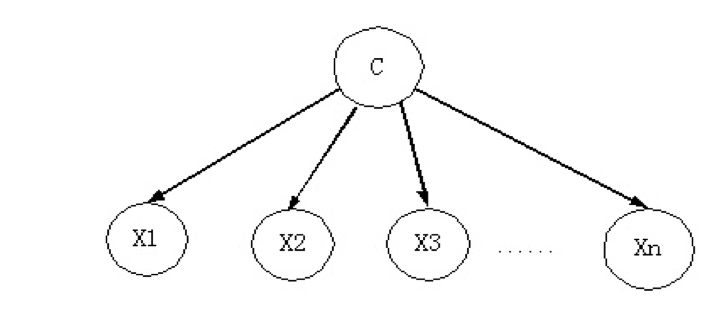
\includegraphics[width=.5\textwidth]{bays1.png}
\caption{朴素贝叶斯过滤器结构图}
\label{fig:logo}
\end{figure}
朴素贝叶斯过滤器主要是利用先验概率求出后验概率,并且根据训练样本集构造过滤器,过滤器根据邮件的后验概率对文本进行分类。
\section{贝叶斯过滤器}
Bogofilter是目前比较流行的贝叶斯过滤器,它的主要原理是朴素贝叶斯理论。Bogofilter建立垃圾邮件和非垃圾邮件贝叶斯概率模型,在贝叶斯原理的实现上,加入了Paul Graham 关于垃圾邮件的过滤理论。该理论大体思想是,在已知的垃圾邮件中,一些单词出现的频率较高,而在合法邮件中,另一些单词出现的频率较高。运用一些众所周知的数学知识,对于每个单词,可以生成一个”垃圾邮件指示性概率”。根据消息中所办含一组词,可以用另一个简单的数学公式来确定文本消息的整体垃圾邮件概率。

Bogofilter将由空格隔开的单词作为特征,并且对特征进行更加严格的定义,譬如,去除单纯包含数字的特征,对于\$20-25这种形式的价格范围,被标记为两个关键词,\$20和\$25等。Bogofilter还使用了平滑技术,来加强过滤器的过滤精度。

 在过滤效率上,Bogofilter采取有效的数据表示,和高效的数据存储技术,获得比较高的过滤效率。Bogofilter使用高性能的Berkerly DB 数据库。Berkerly DB是历史悠久的嵌入式数据库系统,其小巧,可靠,性能高。Berkerly DB 比SQL SERVER 等数据库性能要高10-20倍。
\section{贝叶斯过滤器的优缺点}
朴素贝叶斯算法,其条件概率独立假设,虽然忽略了特征的条件依赖性,但是,在许多实际应用领域中取得了很好的结果,而且其计算简单,降低了算法的复杂性。

 不同与对普通文本的分类,在邮件过滤方面,朴素贝叶斯过滤器也存在一些缺陷。因为邮件分类是一种二类分类问题,且邮件不同于普通文本,有其独特的结构。例如:邮件由邮件头和邮件正文组成,普通的文本分类朴素贝叶斯算法会将邮件头和邮件正文不加区别,而没有考虑到邮件头和邮件正文对邮件类别影响程度的不同。另外邮件分类是一种二类分类问题,两个分类之间是互相影响的,例如合法邮件的误判率低,而非法邮件的误判率高,说明判定一封邮件为非法邮件的阈值过高,为合法邮件的阈值过低。而在普通文本分类时,朴素贝叶斯只是挑选后验概率最大的分类作为文本类别,没有考虑到两类分类中,阈值相关问题。
 
针对朴素贝叶斯在邮件过滤问题上暴露的缺点,我们对朴素贝叶斯过滤器的相关流程做出一系列改进,改进的内容在第四章会有详细描述。
\section{朴素贝叶斯邮件过滤器的扩展}
朴素贝叶斯过滤器在样本学习阶段,通常采用被动学习的方式,这种学习方式没有样本筛选的过程,算法复杂性小,但是这种学习方式造成过滤精度依赖样本的顺序性。

本节提出一种主动学习的贝叶斯过滤器作为普通贝叶斯过滤器的一种扩展。在分类决策阶段。朴素贝叶斯算法是一种基于最小错误率的决策方法,这种决策方法把各种类别的错误判断一视同仁,但是在邮件过滤中,合法邮件误判更应该引起人们重视,所以在此提出最小风险贝叶斯算法,以风险高低作为类别的决策依据,也是在决策阶段对于朴素贝叶斯邮件过滤器的一种扩展。
\subsection{最小风险贝叶斯}
朴素贝叶斯算法是基于最小错误率的决策方法。但是,在邮件的分类与过滤中,合法邮件与垃圾邮件具有不同的特性。合法邮件被判定为垃圾邮件可能给用户带来更大的损失。因此,考虑到各种错误造成的损失不同,可采用最小风险的贝叶斯决策对邮件进行过滤和分类。

基于最小风险的贝叶斯过滤算法是一种特殊的贝叶斯算法,它把邮件分为两类,即合法邮件和非法邮件。最小风险贝叶斯算法是用来增强前面描述的朴素贝叶斯过滤器的性能,降低邮件过滤的风险,以得到一个风险最小的邮件过滤器,是对朴素贝叶斯进行的修正。最小风险贝叶斯的邮件过滤算法,对合法邮件判断为非法邮件以及非法邮件判断为合法邮件定义不同的风险,选择风险最小的决策类别,可以有效降低错误决策造成的损失。
\subsection{主动学习贝叶斯}
根据分类学习对训练样本的处理方式,可将分类模型分成两类:被动分类和主动分类模型。被动分类模型也称”从样本中学习” ,它随机的选择训练样本,被动地接受这些样本的信息,如图2-2。它对于具有严格序关系的训练样本来说是必要的,也是不可改变的。然而绝大部分分类学习中都认为训练样本是独立同分布的,这种被动的学习显示出明显的不足:1)顺序的处理训练样本往往会使学习的过滤器具有顺序相关性,对数据过分敏感;2)遇到噪音样本时,会使这种噪音一直传播下去,影响分类精度3)缺乏综合未带标注样本信息的能力。在学习分类模型中,未带标注的样本往往包含有助于分类的信息。在这种情况下,选择好的未带标注的样本,把它加入到当前的过滤器中是相当重要的。主动分类模型对训练样本的选择是主动的,它选择最有利于过滤器性能的样本来训练过滤器,属于更高层次的,具有潜意识的学习,如图2-3
\begin{figure}[htbp]
\centering
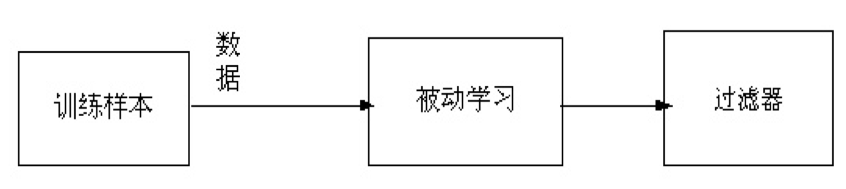
\includegraphics[width=.9\textwidth]{bays2.png}
\caption{被动学习模式}
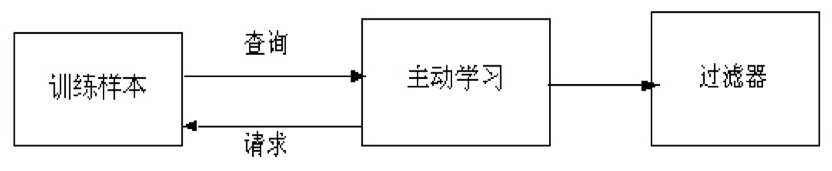
\includegraphics[width=.9\textwidth]{bays3.png}
\caption{主动学习模式}
\label{fig:logo}
\end{figure}

由于贝叶斯网络分类具有增量学习的特性,它更适宜主动学习,在增量地分类和增量学习概率分布方面可以大大的提高效率.传统的学习算法使用给定的训练样本学习分类参数,它所处理的训练样本必须是带有类别标注的,并且一般都假定各训练样本是独立同分布的.相反,主动学习算法在侯选样本集中主动选择测试样本。
\section{邮件评测}
为了能对不同的垃圾邮件过滤算法进行评测,必须有一个可供比较的平台。这包括公共的评测语料,统一的过滤模式和统一的评价方法。
\subsection{邮件过滤语料库}
文本分类问题研究的成功开展,很大程度得益于规范,手工标注类别,公共的文本分类语料库,例如路透社语料,已经成为了标准的测试平台。但是垃圾邮件的语料问题更加复杂,因为邮件涉及到了用户的隐私问题。因此,很多研究者所使用的邮件语料都是私人的,不公开的。这样不同的研究者使用不同的测试语料,所得到的结果就没有很好的可比性,这在一定程度上影响了邮件过滤研究的进展。

垃圾邮件的获得是比较容易的,目前也有很多团队和网站对研究者提供免费下载的垃圾邮件语料,比如SpamArchive.orgAn,nexia.Org等。合法邮件的获得就比较困难,由于邮件使用者往往由于隐私而不愿意公开自己的邮件。所以研究者一般有三种方法获得可以公开的合法邮件语料:

$\blacksquare$ 从新闻组News Group ,邮件列表或者论坛获取文件作为合法邮件。SpamAssassin语料。Ling-Spam语料就是采用这种方法。

$\blacksquare$ 将邮件进行特征选择和向量化处理,公开每个邮件所对应得向量。Spambase就是这种方式。

$\blacksquare$ 将邮件进行编码或者加密,公开的是加密后的邮件。比如PU语料库就是采用这种方式。
本文对算法作进行试验采用了两种邮件集,一个的是全国搜索引擎和网上信息挖掘学术研讨会(SEWM 2008)中文Web信息检索评测中的垃圾邮件过滤评测中,华南理工大学负责收集研制的SEWM 2008邮件集;一个是文本检索会议(text  retrieal conference,简称TREC )提出的trec07p语料库。

SEWM 2008邮件集中的正常邮件来源于三个部分。一个是项目组成员提供的私人邮件;一个是公开邮件群发送的实际邮件;还有按照实际私人邮件和公开邮件的主题、词频、附件等分布特征,通过Internet抓取到邮件内容合成的电子邮件。 其垃圾邮件全部来源于本实验室实际运行邮件服务器上所截获以及用户报告的垃圾邮件,经过部分去重并与其他公开垃圾邮件样本集进行对照后挑选得到。 最后构造的private邮件集中总共包含99054封邮件,其中有24054封正常邮件,75000封垃圾邮件

文本检索会议(text  retrieval conference,简称TREC )从2005年开始构造邮件数据集,其中Trec06数据集加入了中文语料。而Trec07语料总共包括75339封邮件,其中25,220封ham和50119封spam。
\subsection{邮件过滤模式}
邮件过滤模式包括两种,一种是离线过滤模式,一种是在线过滤模式。离线过滤模式是先通过训练邮件集的训练,得到邮件过滤模型,再通过训练得到的邮件模型,对待测试邮件集进行过滤。在线过滤模型运用用户反馈在线更新模型库,然后通过更新的模型判断邮件类别。

 通过对实际的反垃圾邮件应用需求进行抽象,得到的电子邮件在线过滤模式如图6-1所示,以过滤器和学习器为中心分为过滤和学习两部分。过滤器根据在线更新的知识库,过滤按时间顺序输入的邮件流,对每个邮件做出Spam 或Ham 的判断。学习器根据客户反馈对每个邮件的过滤结果进行在线学习,学习的结果进一步精化过滤器的知识库,使得下一个邮件到来时能提高过滤器的性能。
\begin{figure}[htbp]
\centering
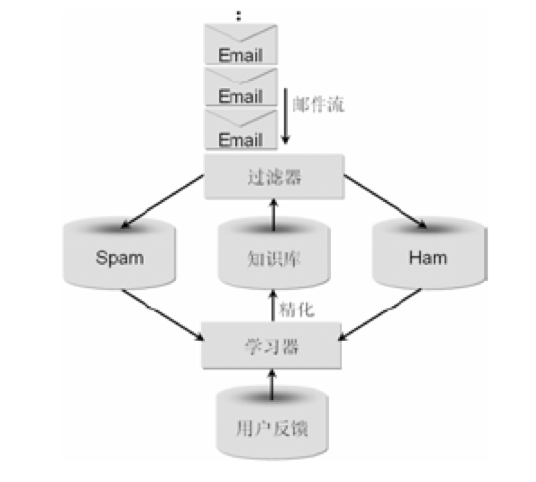
\includegraphics[width=.8\textwidth]{bays4.png}
\caption{电子邮件在线过滤模式}
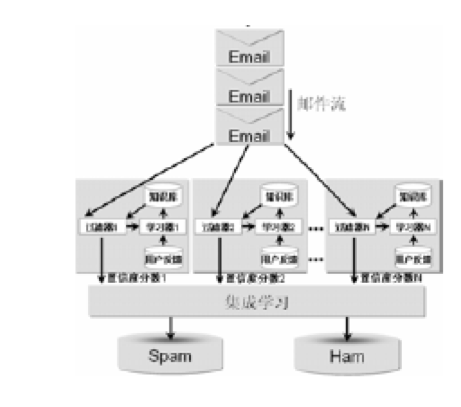
\includegraphics[width=.8\textwidth]{bays5.png}
\caption{离 线 过 滤 模 式}
\label{fig:logo}
\end{figure}
随着过滤器的不断使用和客户不断反馈,学习器逐渐收集了很多带有客户反馈的邮件,每次学习时都可以使用当前收集到的带反馈邮件集进行训练。在TREC Spam 任务中,采用标准答案(Golden Standard)来模拟客户反馈。由于实际应用中客户不一定能够及时正确的给出反馈,所以TREC Spam 任务用立即反馈和延时反馈两种类型来模拟不同的客户反馈时机。立即反馈对于过滤后的每一个邮件能够立刻得到标准答案,通过学习可以马上精化知识库。延时反馈对于过滤后的邮件有可能要过一段时间才能得到答案,甚至永远得不到答案或是得到错误的答案。
\subsection{评价体系}
垃圾邮件过滤的性能评价通常借用文本分类的相关指标。具体地,假设待测试的邮件集合中共有N封邮件,一个垃圾邮件过滤系统的判定结果如下表所示:
\begin{table}[!htbp]
\centering
\begin{tabular}{|c|c|c|}% 通过添加 | 来表示是否需要绘制竖线
\hline  % 在表格最上方绘制横线
&实际为垃圾邮件&实际为合法邮件\\
\hline  %在第一行和第二行之间绘制横线
实际为合法邮件&A&B\\
\hline % 在表格最下方绘制横线
系统判定为合法邮件&C&D\\
\hline % 在表格最下方绘制横线
\end{tabular}
\end{table}

其中,$N=A+B+C+D=N_s+N_h$,其中$N_s=A+C$为实际的垃圾邮件数目,为实际的合法邮件数目。

在评价体系中,本节主要介绍三种评价体系:沿用传统文本分类的评价系统,	ROC 评价方法,以及TREC评测方法。

$\blacksquare$ 沿用传统文本分类的评价系统
定义如下几个评价指标来衡量不同垃圾邮件过滤系统的性能:
(1) 召回率(Recall) :$R=\frac{A}{A+C}=\frac{A}{N}$ ,即垃圾邮件的检出率。这个指标反映了过滤系统发现垃圾邮件的能力,召回率越高,”漏网”的垃圾邮件就越少。

(2)正确率(Precision):$R=\frac{A}{A+B}$ 即垃圾邮件检对率。正确率反应了过滤系统”找对”垃圾邮件的能力,正确率越大,将非垃圾邮件误判为垃圾邮件的数量越少。

(3)精确率(Accuracy):$Accur=\frac{A+D}{N}$ ,即对所有邮件(包括垃圾邮件和合法邮件)的判对率。

(4)错误率(Error rate):$Err=\frac{B+C}{N}=1 Accur$ 即对所有邮件(包括垃圾邮件和合法邮件)的判错率。

(5)F值:$F=\frac{2PR}{R+P}$ F实际上是召回率和正确率的调和平均,它将召回率和正确率综合成一个指标。

除此之外,垃圾邮件过滤中还常常采用虚报率(Fallout)、漏报率(Miss rate)等指标。

另外,我们在前面提到,在实际的垃圾邮件过滤中,人们往往不希望将合法邮件误判成垃圾邮件。为了表示不同情况下垃圾邮件系统的代价。Androutsopoulos等人提出了代价因子CR的概念。设合法邮件误判为垃圾邮件的损失为是垃圾邮件判为合法邮件的入倍。则可以定义:

垃圾邮件系统的加权错误率 $WErr=\frac{B+C}{N_h+N_s}$

在没有任何垃圾邮件过滤器(即所有的垃圾邮件被当成合法邮件)的情况下,可以计算基准的加权错误率: $WErr=\frac{N_s}{N_1+N_s}$

于是,代价因子$TCR=\frac{WErr_b}{WErr}=\frac{N_s}{B+C}$,TCR越高,表明当前垃圾邮件过滤系统的成本越低。

$\blacksquare$ ROC评价方法
在现实问题当中,代价因子CR往往是无法确定的,甚至是变化非常大的。而且合法邮件和垃圾邮件的数目之比N : NS,这个数值也是无法确定并且变化非常大的。而上面所述的评价方法只能评价算法在某一个具体条件下的性能。所以,对垃圾邮件问题来说,必须使用一种能反映各种条件下算法性能的评价方法,ROC就是这样的方法。

在ROC图中,横轴表示ham misclassification rate(hmr),即将合法邮件漏判率,对应于$WErr=\frac{B}{B+D}$;纵轴表示spam misclassification rate(smr),即垃圾邮件漏判率,对应于$WErr=\frac{C}{A+C}$,即1-Recall。。在ROC中,每一个点都对应这样一个(hmr,smr)点。调整问题条件,每个过滤器都会得到一系列这样的点,最后形成一条ROC曲线。如图 3-6中的红色曲线。

在ROC图中的两个点,左上方的点总是比右下方的点更优,因为左上方的点有更小的hmr,和更小的smr。

对于两个算法来说,ROC曲线越靠左上的算法性能越优。对于机器学习算法来说,一般可以通过调整阈值的方法来得到ROC曲线。在垃圾邮件过滤算法中,产生ROC 曲线方法如下:对于一批测试样本中的每封邮件,使用过滤器依次对其进行打分产生一个score值,反映该邮件为spam的可能性。若确定了所有邮件的score值,我们可以通过动态调整阈值t来获得每种可能的hmr%以及对应的smr%,即通过动态调整阈值t,我们可以将smr%表示成hmr%的某个函数,从而画出ROC曲线图
\begin{figure}[htbp]
\centering
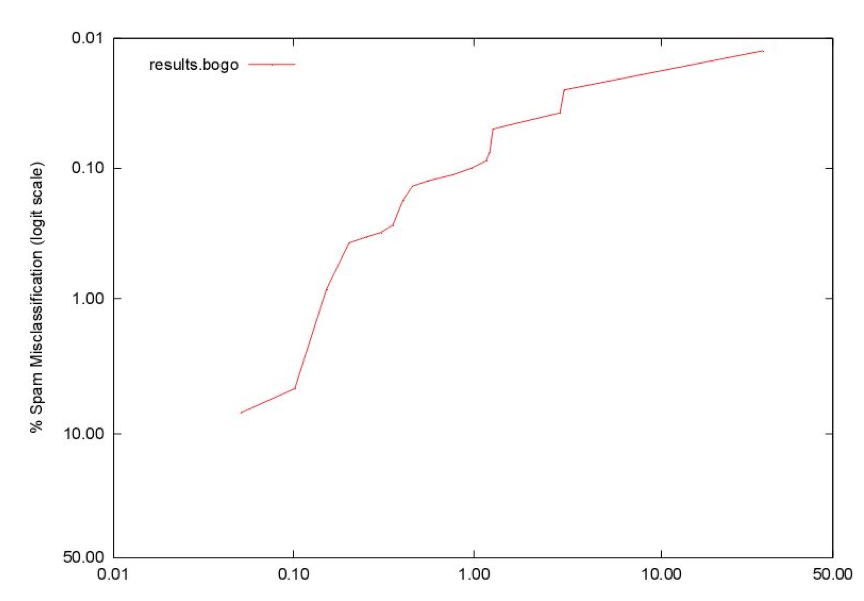
\includegraphics[width=.9\textwidth]{bays6.png}
\caption{ROCA 图}
\label{fig:logo}
\end{figure}

$\blacksquare$ TREC 2005 SPAM track 的评测方法

文本检索会((Text Retrieval Conference, TREC)是目前国际上信息检索领域一年一度的学术交流与系统评测活动,由美国NIST(National Institute of Standards and Technology)、DARPA(Defense  Advanced  Research  Projects  Agency)、DARDA(US Department of Defense Advanced Research and Development Activity)等单位共同主办。TREC在2005年新引入了垃圾邮件过滤器的评测。TREC 2005 SPAM track主要使用了4种评测方式:

$\bullet$ hm\%: 合法邮件漏判率hmr(ham misclassification rate),合法邮件被判成垃圾邮件的比例。

$\bullet$ sm\%:  垃圾邮件漏判率smr(spam misclassification rate),垃圾邮件被判成合法邮件的比例。

$\bullet$ 以hm\%为横坐标,以sm\%为纵坐标,取不同的阈值t时,做ROC曲线

$\bullet$ (1-ROCA)\%: ROC曲线的上方的面积。越小越好,物理意义是过滤器给一个随机的合法邮件的spam打分,等于或大于过滤器给一个随机的垃圾邮件的spam打分的概率。

这四个指标数值越小,表示垃圾邮件过滤系统性能越好。


\section{本章小结}
本章介绍了贝叶斯垃圾邮件过滤算法以及邮件评测的相关内容。第一节到第四节主要是贝叶斯算法的一些介绍。其中详细介绍了贝叶斯定理,以及贝叶斯定理在邮件过滤中的应用:朴素贝叶斯算法。并且通过描述朴素贝叶斯算法的优缺点,引出了最小风险贝叶斯算法和主动学习贝叶斯算法,并且介绍了最小风险贝叶斯算法和主动学习贝叶斯算法的基本原理。第五节到第七节主要介绍了垃圾邮件过滤的几种常用技术以及评价垃圾邮件过滤方法所采用的邮件集和评价体系。垃圾邮件过滤技术从简单的黑白名单技术开始,介绍到本论文所采用的贝叶斯过滤技术。本文采用的邮件集有两种,一种是trec07语料库,一种是sewm2008语料库。在评价体系上,本章主要介绍了TREC 2005 SPAM track 运用的评价标准,重点介绍了ROC评价方法。








\chapter{朴素贝叶斯过滤器的改进}

\section{贝叶斯分类流程}
上章描述了几种贝叶斯算法的原理以及优缺点,本节介绍基于贝叶斯算法的垃圾邮件过滤流程。

1) 收集一定数量的垃圾邮件和正常邮件,建立垃圾邮件集和正常邮件集。

2) 对垃圾邮件集和正常邮件集中的邮件进行内容解析,并提取关键词,

3) 建立两个哈希表分别用于存储垃圾邮件集和正常邮件集中的关键词和出现的次数。

4) 计算处理后的每一个关键词的概率。

5) 对于需要判定的邮件,提取其关键词,计算这些关键词的联合概率。

6) 设定一个判断垃圾邮件的阀值,若计算出的联合概率大于该值,则判定为垃圾邮件。反之,则判定为正常邮件。

\section{贝叶斯邮件过滤器的改进方面}
上节描述了贝叶斯的分类流程,为了更好的用贝叶斯算法进行垃圾邮件过滤,我们在以下几个方面对贝叶斯算法进行改进:

(1)	文本表示

在普通文本分类贝叶斯算法中,文本用词语或者短语表示。因为词语和短语是能代表语意的最小单位。但是在垃圾邮件中,垃圾邮件制造者为了避免被过滤,,采用垃圾变种词语代替垃圾词语。譬如:垃圾词语:法轮功,其变种词语可以是法!!轮===功@。我们采用指纹来表示文本,能够较好的辨别变种词汇,指纹特征会在3.3节中进行详细描述。

(2)	特征选择

普通贝叶斯文本分类算法在特征选择上大多采取信息增益,期望交叉熵等算法。通过对贝叶斯原理的分析,发现特征的分布情况与特征代表类别能力息息相关,因此提出一种新的特征选择方法,基于类条件分布的算法,具体会在第4.4节中给出描述

(3)	 阈值动态调整

朴素bayes通过学习来构造模型参数,其学习过程是一个由浅至深的过程。最开始,学习的样本少,导致模型参数不够精确,判断一封邮件为垃圾邮件的分数也不准确,随着学习的深入,判断的准确性也随之慢慢提高.因此,我们提出阈值动态调整算法,来适应不断提高的邮件类别判断准确性.这部分在3.5节中会有详细描述。

\section{文本表示}
\subsection{词语特征项}
在文本分类领域中,通常采用向量模型(VSM )来表示文本,一篇文本可以表示成为一个n维向量$(t_1,t_2,t_3,...,t_n)$。其中$t_i(i=1,...,n)$表示第i个特征项的权重。

在英文文本中,特征项通常定义为用空格键、制表符或各种标点符号及重音符号等隔开的一系列连续字符串,一般情况下,特征项就是有意义的单词或词组。在字符处理过程中,所有的大写字母转换成小写字母。所有空格键、制表符、换行符和各种标点符号及重音符号都删除掉。

在中文文本中,特征项可以是字、词、短语或者某种概念,在中文文本中主要指经过分词处理后得到的词汇。但是对多封垃圾邮件进行相似度比较的时候,我们发现在同类垃圾邮件出现较高的是一些文本块短语。并且现在的垃圾邮件制造者为了避免被过滤,经常采用垃圾词汇变种的方法来防止被过滤,譬如:在垃圾邮件中经常出现以下变种词语:法¥¥轮\%\%\%\%功,功999产**党的暴———政等等,所以,在日新月异的垃圾邮件变种中,单纯的采用词语特征已经不能满足要求。

\subsection{指纹散列特征项}
指纹应用在相似邮件的比较上。在比较两封邮件是否相似的时候,可以先把两封邮件划分为很多个文本块(实际上也是子字符串),如果两封邮件是相似的,那么它们之间一定包含很多公有的文本块。而且这些文本块之间的比较操作,是精确比较,因此就可以用散列方法来进行优化。在文献[5]中就提出了一个观点:在这种应用场合中,可以用一组散列值来代表一个文件(而不是一个散列值)。这样的一组散列值在以下的论述中就称为邮件的“指纹”。

其中的每一个散列值, 称为指纹的一个元素, 可以从邮件中的一个片断中提取。按照这种思路, 从一封邮件中提取指纹的步骤可以这样进行:

(1) 把一封邮件看作n个文本块的集合;

(2) 引入一个散列函数,计算每个文本块的散列值;

(3) 按照一定规律,筛选出一些散列值,作为这封邮件的特征代码表。或者称为邮件的”指纹”。

这一节中介绍的是一种通用的思路。通过指定不同的文本块划分方法、选用不同的散列函数或者对散列值采用不用的筛选条件,按照上述步骤可以生成多种指纹算法。

\subsection{一种指纹算法}

下面介绍一种用于最初用于文件管理领域的指纹算法。这种算法的效率很高,因此在国外最近的一些反垃圾邮件研究中仍然采用了这种算法。

下面描述指纹的计算过程。

 (1) 文本块的划分。这种算法从文档的每一个位置开始,都取出一度为 k的子字符串。这样在一个长度为 n 的文档中,一共包含n-k+1个这样的字符串。
 
(2) 散列函数采用了Karp-Rabin算法[7]

  Karp-Rabin算法是一种著名的模式匹配算法。它通过把字符串的匹转换成相应的整数的匹配,而大大提高了匹配的效率。这种算法在计算”相应的整数”时,对长度为 k的子字符串 用了以下的散列函数:
\begin{equation}
 H_i=t_i*p^{k-1}+t_{i+1}*p^{k-2}+...t_{i+k-2}*p^+t_{i+k-1} ~~~~~~~~~~~~~~(P\in N)
\end{equation}
如果对每一个子字符串的散列值都从头开始计算,代价是很高的,karp-Rabin算法采用了以下方法来进行简化:
\begin{equation}
 H_{i+1}=p*H_i+t_{i+k} ~~~~~~~~~~~~~~t_i*p^k
\end{equation}

由于$P^k$是一个常数,所以采用了以上的简化方法以后,每个指纹元素 Hi的计算代价就只有两次乘法和加减法各一次,是非常低的。

 上述计算方法得出的指纹元素往往会超过一个整数的表示范围,因此实际应用的时候可以对上述计算结果取模,或取计算结果中最低的几个位。
\section{特征选择}
特征选择是文本分类中的重要研究领域,其目的是要在一个训练文本的众多的特征中选择出能代表该文本及与该文本所属类别的若干重要特征。特征选择考虑的首要问题是特征与类之间的关系,即选择出来的特征是否真正代表一个类。

  常见的特征选择的方法有:期望交叉熵,信息增益法,互信息法。卡方检验法,主成分分析发等。这些方法或者从信息论的角度或者从统计分析的角度,来找出含有信息量最大或者影响显著的特征,而忽略掉其余的特征,达到特征约简的目的。
\subsection{信息增益}
信息增益,是决策树技术中经常采用的一种选择最佳节点的方法。它利用的是信息论中熵的概念。在信息论中,熵是对事物不确定性的一种度量。它是以各个特征取值情况来划定学习样本空间,根据所获得信息增益的多少来选择有效的特征。特征的信息增益如下所示:
\begin{equation}
 IG(t)=\sum_{i=1}^{n}p(c_i)+p(t)\sum_{i=1}^{n}p(c_i|t)\log p(c_i|t)+p(\bar{t})\sum_{i=1}^{n}p(c_i|\bar{t})\log p(c_i|\bar{t})
\end{equation}
其中$p(c_i)$为文档集中出现类别$c_i$的概率;p(t)为特征出现在文档集中的概率;$p(c_i|t)$表示当t出现在文档集中时,文档属于$c_i$的概率;$p(c_i|\bar{t})$表示当t不出现在文档集中时,文档属于$c_i$的概率。

特征在文本中是否出现都将为文本分类提供信息,计算不同情况下的条件概率已确定提供的信息量的大小。信息增益利用特征取值情况划分训练样本空间,根据所获得信息量的多少选择特征。在进行特征选择时,选择信息增益大的那些特征。该特征选择方法存在的问题是如果一个特征在类中出现,而在类中不出现,这个特征本身非常重要,但是对各log值求和之后相抵消,结果为0,与某些词无法区分,解决这个问题有两种方法:一是对log值取绝对值,二是略去log值小于0的情况。此外,该方法计算也比较复杂。

\subsection{实验及分析}
为了比较三种特征选择方法对分类精度的影响,我们对分别采用三种特征选择方法的过滤器采用离线和在线两种过滤模式来进行过滤。其中在线过滤模式在trec07 p 邮件集上进行,并且采用在线立即反馈模式,离线模式在 sewm 2008 公开集上进行。

在特征选择标准上,提取的关键特征的个数对过滤精度也有一定的影响,因此我们分别提取特征数为8,10,15上,并且比较三种特征选择方法在邮件过滤精度上的区别。首先比较在trec07 p上采用在线及时反馈的实验,实验使用TREC 的Spam 评测工具,实验结果如下所示:



\begin{table}[!htbp]
\centering
\begin{tabular}{|p{3cm}|p{3cm}|p{3cm}|p{3cm}|}% 通过添加 | 来表示是否需要绘制竖线
\hline  % 在表格最上方绘制横线
评价参数|特征选择方法&信息增益&期望交叉熵&类条件分布(ccd值)\\
\hline  %在第一行和第二行之间绘制横线
Ham\%&2.39(1.76-3.16)&1.18 (1.05-1.32)&1.42 (0.95-2.05)\\
\hline % 在表格最下方绘制横线
Spam\%&1.10 (0.88-1.35)&0.87 (0.79-0.96)&0.16 (0.09-0.28)\\
\hline % 在表格最下方绘制横线
Lam\%&1.62 (1.37 - 1.91)&1.01 (0.95 - 1.08)&0.48 (0.34 - 0.69)\\
\hline % 在表格最下方绘制横线
1-ROCA\%&0.3509 (0.1166 - 1.0512)&0.3728 (0.1699 – 1.8844)&0.2963 (0.1453 – 1.
4129)\\
\hline % 在表格最下方绘制横线
\end{tabular}
\caption{特征选取个数为8的三种算法在线过滤精度}
\end{table}


\begin{table}[!htbp]
\centering
\begin{tabular}{|p{3cm}|p{3cm}|p{3cm}|p{3cm}|}% 通过添加 | 来表示是否需要绘制竖线
\hline  % 在表格最上方绘制横线
评价参数|特征选择方法&信息增益&期望交叉熵&类条件分布(ccd值)\\
\hline  %在第一行和第二行之间绘制横线
Ham\%&1.16(1.13-1.42)&1.20(1.03-1.29)&1.32(1.05-1.00)\\
\hline % 在表格最下方绘制横线
Spam\%&0.86 (0.75-0.90)&0.86(0.79-0.95)&0.14(0.05-0.26)\\
\hline % 在表格最下方绘制横线
Lam\%&1.02 (0.94 - 1.11)&1.00 (0.93 -1.07)&0.39 (0.35 - 0.44)\\
\hline % 在表格最下方绘制横线
1-ROCA\%&0.2986(0.2673 -0.3444)&0.2739 (0.2563 – 0.3346)&0.1363 (0.1053 – 0.
3129)\\
\hline % 在表格最下方绘制横线
\end{tabular}
\caption{特征选取个数为10的三种算法在线过滤精度}
\end{table}


\begin{table}[!htbp]
\centering
\begin{tabular}{|p{3cm}|p{3cm}|p{3cm}|p{3cm}|}% 通过添加 | 来表示是否需要绘制竖线
\hline  % 在表格最上方绘制横线
评价参数|特征选择方法&信息增益&期望交叉熵&类条件分布(ccd值)\\
\hline  %在第一行和第二行之间绘制横线
Ham\%&2.15(1.56-3.11)&1.17(1.04-1.33)&1.40 (0.97-2.00)\\
\hline % 在表格最下方绘制横线
Spam\%&0.96(0.78-1.24)&0.88(0.78-0.95)&0.88(0.78-0.95)\\
\hline % 在表格最下方绘制横线
Lam\%&1.32(1.27 - 1.85)&1.32(1.27 - 1.85)&1.32(1.27 - 1.85)\\
\hline % 在表格最下方绘制横线
1-ROCA\%&0.3423(0.1166- 1.0512)&0.3423(0.1166- 1.0512)&0.2567(0.1343 – 1.
3879)\\
\hline % 在表格最下方绘制横线
\end{tabular}
\caption{特征选取个数为15的三种算法在线过滤精度}
\end{table}

\newpage
实验结果显示,不论是在线立即反馈还是离线模式,采取同一个邮件过滤算法时,特征选取个数不同,垃圾邮件过滤精度不同。当特征选取个数为10时,不论是使用信息增益,期望交叉熵,还是类条件分布特征选择算法时,其邮件过滤精度要好于特征选取个数为8和15的算法。这表明特征选择的个数并不是越多越好;特征选取多,不仅增加了计算的难度,而且也会带来一些类别代表能力不强,类别模拟两可的噪音特征的加入。又由于文本内容中各个词汇之间本来就不是完全独立的,朴素贝叶斯方法的前提是假设特征之间相互独立,所以当特征值提取数量增加之后,特征值之间相互依赖的机会增加,独立性变小。但是选取的特征太少,使得分类只片面考虑到部分的特征,忽略掉了很多对分类影响大的特征,导致分类准确性降低。

\section{改进的朴素贝叶斯邮件过滤流程}
本章第二节到第六小节描述了对朴素贝叶斯算法的几个方面的改进,本节总结这些改进方法,并将这些改进方法运用到朴素贝叶斯邮件过滤上。 

改进后的朴素邮件过滤算法的流程图如下所示:
\begin{figure}[htbp]
\centering
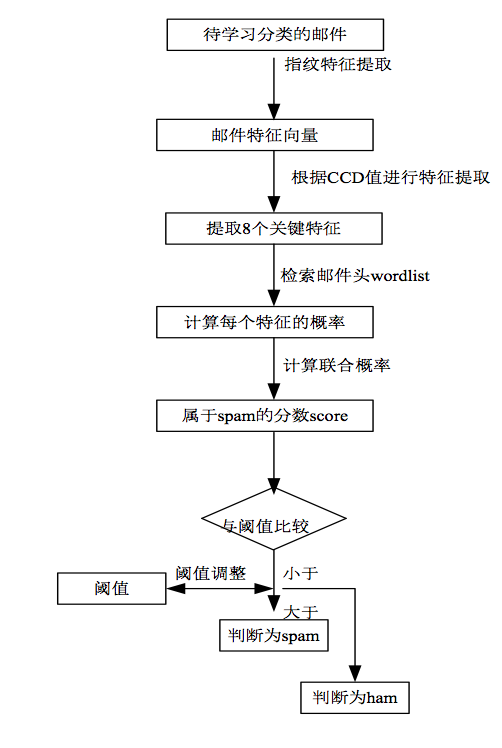
\includegraphics[width=.8\textwidth]{bays7.png}
\caption{改进朴素贝叶斯流程图}
\label{fig:logo}
\end{figure}

\newpage

\begin{lstlisting}[language=python]
<strong>'''''******************************* 
  Copyright (C), 2015-2020, cyp Tech. Co., Ltd. 
  FileName:           朴素贝叶斯实例.cpp 
  Author:             cyp      
  Version :           v1.0           
  Date:               2015-10-21 上午10:38 
  Description:        利用朴素贝叶斯原理对邮件进行分类      
  Function List:       
    1.  createVocalList:计算输入各集的并集,且每个元素是unique 
    2.  setofWords2Vec:  运用词集方式将数据预处理 
    3.  bagofWords2Vec:  运用词袋方式将数据预处理 
    4.  trainNB0:       训练数据 
    5.  classifyNB:      对email进行分类 
    6.  test             相当于主函数,训练模型并测试 
********************************************'''  
  
  
'''''*************************************** 
需要导入的模块 
********************************************''  
import random  
import math  
import numpy as np  
import os  
  
'''''********************************************* 
  Function:        createVocalList 
  Description:     计算输入各集的并集,且每个元素是unique 
  Calls:            
  Called By:       test 
  Input:           dataSet输入的数据集,及单词向量集 
  Return:          返回输入数据集的并集,返回数据的数据类型是list 
                   表示出现过的单词 
************************************************'''  
def createVocalList(dataSet):  
    vocalSet = set([])                  #创建一个空集  
    for data in dataSet:  
        vocalSet = vocalSet | set(data) #利用set的特性求两个集合的并集  
    return list(vocalSet)               #以list的方式返回结果  
      
      
'''''******************************************** 
  Function:        setofWords2Vec 
  Description:     判断的向量的单词是否在词库中是否出现,如果出现 
                   则标记为1,否则标记为0 
  Calls:            
  Called By:       test 
  Input: 
                   vocabList: 
                   词库,曾经出现过的单词集合,即createVocalList 
                   inputSet: 
                   测试的单词向量 
  Return:          returnVec是一个同vocalList同大小的数据,
  如果inputset单词 
                   出现在vocalList则将returnVec对应的位置置1,否则为0 
************************************************'''  
def setofWords2Vec(vocalList,inputset):  
    returnVec = [0]*len(vocalList)         
    #同vocalList同大小的list,开始假设每个单词都没出现,即全为0  
    for word in inputset:                                          
        if word in vocalList:        #如果输入的单词出现在词库中,则置1     
            returnVec[vocalList.index(word)] = 1  
        else:                        #如果没出现在词库中,默认为0,并输出  
            print("the word:%s is not in my Vocabulary!"%word)  
    return returnVec                 #返回结果  
'''''********************************************
  Function:        bagofWords2Vec 
  Description:     统计的单词是否在词库中出现频率 
                  
  Calls:            
  Called By:       test 
  Input: 
                   vocabList: 
                   词库,曾经出现过的单词集合,即createVocalList 
                   inputSet: 
                   测试的单词向量 
  Return:          returnVec是一个同vocalList同大小的数据,对应位置 
                    表示该单词出现的个数 
***********************************************'''  
def bagofWords2Vec(vocalList,inputset):  
    returnVec = [0]*len(vocalList)         
    #同vocalList同大小的list,开始假设每个单词都没出现,即全为0  
    for word in inputset:                                          
        if word in vocalList:        #如果输入的单词出现在词库中,则加1     
            returnVec[vocalList.index(word)] += 1  
    return returnVec                 #返回结果  
'''''****************************************** 
  Function:        trainNB0 
  Description:     统计侮辱性email出现概率,侮辱性邮件各单词出现的概率,非 
                   侮辱性email各单词出现概率 
  Calls:            
  Called By:       test 
  Input: 
                   trainDataSet:参与训练的数据集,
                   即setofWords2Vec返回数据的集合 
                   trainLabels:训练数据的标签 
  Return:           
                    pShame:侮辱性email 
                    p0Vect:非侮辱性email中单词出现的概率 
                    p1Vect:侮辱性email中单词出现的概率 
********************************************'''  
def trainNB0(trainDataSet,trainLabels):  
    numTrains = len(trainDataSet)     #训练数据的组数  
    numWords = len(trainDataSet[0])   #每组训练数据的大小  
    pShame = sum(trainLabels)/float(numTrains)  
    #标签中1表示侮辱,0表示非侮辱,故上述统计侮辱性email出现概率  
    #zeros(numWords)表示1*numWords数组,非numWords*numWords数组  
    #p0Num = np.zeros(numWords)     #存储统计非侮辱性邮件各单词出现频率  
    #p1Num = np.zeros(numWords)         #存储统计侮辱性邮件各单词出现频率  
    #p0SumWords = 0.0                  #非侮辱性邮件中单词总数  
    #p1SumWords = 0.0                  #侮辱性邮件中单词总数  
    #为了防止与0相乘,故初始化为1,因为两者的初始化一样,所以不影响结果  
    p0Num = np.ones(numWords)        #存储统计非侮辱性邮件各单词出现频率  
    p1Num = np.ones(numWords)           #存储统计侮辱性邮件各单词出现频率  
    p0SumWords = 2.0                    #非侮辱性邮件中单词总数  
    p1SumWords = 2.0                    #侮辱性邮件中单词总数  
    for i in range(numTrains):  
        if trainLabels[i]==1:         #如果为侮辱性email  
            p1Num += trainDataSet[i]  #统计非侮辱性邮件各单词  
        else:  
            p0Num += trainDataSet[i]  #统计侮辱性邮件各单词  
    p0SumWords = sum(p0Num)           #计算非侮辱性邮件中单词总数  
    p1SumWords = sum(p1Num)           #计算侮辱性邮件中单词总数  
    p0Vect = p0Num/p0SumWords         #非侮辱性邮件中单词出现的概率  
    p1Vect = p1Num/p1SumWords         #侮辱性邮件中单词出现的概率  
    return pShame,p0Vect,p1Vect  
      
'''''************************************* 
  Function:        classifyNB 
  Description:     对email进行分类 
  Calls:            
  Called By:       test 
  Input: 
              vec2Classify:要分类的数据 
              pShame:侮辱性email 
               p0Vect:非侮辱性email中单词出现的概率 
             p1Vect:侮辱性email中单词出现的概率 
  Return:           
              分类的结果,1表示侮辱性email,0表示非侮辱性email 
********************************************'''  
def classifyNB(vec2Classify,p0Vect,p1Vect,pShame):  
    #由于小数相乘,会有很大误差,故先求对数再相乘  
    temp0 = vec2Classify*p0Vect   
    temp1 = vec2Classify*p1Vect  
    temp00 = []   
    temp11 = []  
    #分步求对数,因为log不能处理array,list  
    for x in temp0:  
        if x>0:  
            temp00.append(math.log(x))   
        else:  
            temp00.append(0)  
    for x in temp1:  
        if x>0:  
            temp11.append(math.log(x))   
        else:  
            temp11.append(0)  
    p0 = sum(temp00)+math.log(1-pShame)  #属于非侮辱性email概率  
    p1 = sum(temp11)+math.log(pShame)    #属于侮辱性email概率  
    if p1 > p0: #属于侮辱性email概率大于属于非侮辱性email概率  
        return 1  
    else:  
        return 0  
  
'''''********************************************* 
  Function:        text2VecOfWords 
  Description:     从email的string中提取单词 
  Calls:            
  Called By:       test 
  Input: 
                   string: email字符串 
  Return:           
                   单词向量 
**********************************************'''  
def text2VecOfWords(string):  
    import re        #正则表达式工具  
    listOfWolds = re.split(r"\W*",string)  
    #分割数据,其分隔符是除单词,数字外任意的字符串   
    return [word.lower() for word in listOfWolds if len(word)>2]  
    #单词不区分大小写,及全部转换为(小写),滤除没用短字符串  
  
'''''*****************************************
  Function:        test 
  Description:     将数据部分用来训练模型,部分用来测试 
  Calls:           text2VecOfWords 
                   createVocalList 
                   trainNB0 
                   classifyNB 
  Called By:       main 
  Input: 
  Return:           
******************************************'''  
def test():  
    emailList = []               #存放每个邮件的单词向量  
    emailLabel = []              #存放邮件对应的标签  
    cwd = "C:\\Users\\cyp\\Documents\\
    sourcecode\\machinelearning\\my__code\\chapter4\\"  
    for i in range(1,26):  
        #读取非侮辱邮件,并生成单词向量  
        wordList = text2VecOfWords(open(cwd+r"email\ham\%d.txt"%i
        ,encoding='Shift_JIS').read())  
        emailList.append(wordList)#将单词向量存放到emailList中  
        emailLabel.append(0)      #存放对应的标签  
        wordList = text2VecOfWords(open(
        cwd+r"email\spam\%d.txt"%i,encoding='Shift_JIS').read())  
        #读取侮辱邮件,并生成单词向量  
        emailList.append(wordList)#将单词向量存放到emailList中  
        emailLabel.append(1)      #存放对应的标签  
    vocabList = createVocalList(emailList)#由所有的单词向量生成词库  
    trainSet = [i for i in range(50)]     #产生0-49的50个数字  
    testIndex = []                        #存放测试数据的下标  
    for i in range(10):                   #从[0-49]中随机选取10个数  
        randIndex = int(random.uniform(0,len(trainSet)))  
                                          #随机生成一个trainSet的下标  
        testIndex.append(trainSet[randIndex])#提取对应的数据作为训练数据  
        del(trainSet[randIndex])    #删除trainSet对应的值,以免下次再选中  
    trainDataSet = []             #存放训练数据(用于词集方法)  
    trainLabels = []              #存放训练数据标签(用于词集方法)  
    trainDataSet1 = []             #存放训练数据(用于词袋方法)  
    trainLabels1 = []              #存放训练数据标签(用于词袋方法)  
    for index in trainSet:        #trainSet剩余值为训练数据的下标  
        trainDataSet.append(setofWords2Vec(vocabList,emailList[index]))  
        #提取训练数据  
        trainLabels.append(emailLabel[index])  
        #提取训练数据标签  
        trainDataSet1.append(bagofWords2Vec(vocabList,emailList[index]))  
        #提取训练数据  
        trainLabels1.append(emailLabel[index])  
        #提取训练数据标签  
    pShame,p0Vect,p1Vect = trainNB0(trainDataSet,trainLabels)
    #开始训练  
    pShame1,p0Vect1,p1Vect1 = trainNB0(trainDataSet1,trainLabels1)
    #开始训练  
    errorCount = 0.0          #统计测试时分类错误的数据的个数  
    errorCount1= 0.0          #统计测试时分类错误的数据的个数  
    for index in testIndex:  
        worldVec = setofWords2Vec(vocabList,emailList[index])
        #数据预处理  
        #进行分类,如果分类不正确,错误个位数加1  
        if classifyNB(worldVec,p0Vect,p1Vect,pShame) 
        != emailLabel[index]:  
            errorCount += 1  
        worldVec = bagofWords2Vec(vocabList,emailList[index])
        #数据预处理  
        #进行分类,如果分类不正确,错误个位数加1  
        if classifyNB(worldVec,p0Vect1,p1Vect1,pShame1) 
        != emailLabel[index]:  
            errorCount1 += 1  
    #输出分类错误率  
    print("As to set,the error rate is :",
    float(errorCount)/len(testIndex))  
    print("AS to bag,the error rate is :",
    float(errorCount1)/len(testIndex))  
      
'''''************************************ 
  Function:       main 
  Description:    运行test函数 
  Calls:          test 
  Called By:        
  Input: 
  Return:           
*******************************************'''  
if __name__=="__main__":  
    test()</strong>  

\end{lstlisting}

\section{本章小节}
本章首先介绍了朴素贝叶斯算法的分类流程,并且针对其分类流程提出了四个方面的改进在文本表示方面提出了指纹特征;在概率计算方面提出了新的联合概率公式和解本章首先介绍了朴素贝叶斯算法的分类流程,并且针对其分类流程提出了四个方面的改进在文本表示方面提出了指纹特征;在概率计算方面提出了新的联合概率公式和解



\chapter{结论及展望}

垃圾邮件过滤技术是随着垃圾邮件在互联网中的蔓延而产生的一种新技术。垃圾邮件带来了巨大的危害,因此研究高过滤精度的垃圾邮件过滤算法有着重大的现实意义。

本文总结了垃圾邮件的定义,危害,垃圾邮件过滤技术的分类以及垃圾邮件过滤技术的研究现状,并从贝叶斯算法出发详细分析了文本表示方法,特征选择算法,电子邮件的格式标准,以及阈值对垃圾邮件过滤精度的影响。本文还分析了朴素贝叶斯算法在合法邮件误判风险以及反馈学习的优缺点,提出了两种扩展模型。

  在贝叶斯算法的研究上,本文主要做出了如下几点贡献:
  
1.	分析了传统文本分类文本的表示方式,提出了指纹特征。指纹特征相对于词语特征来说,能提取更多的文本信息。

2.	研究特征选择的一般方法,并根据贝叶斯原理,提出基于类条件分布的特征选择方法。

3.	分析电子邮件的结构,根据电子邮件的结构与一般文本的区别,提出集成加权过滤模型。

4.	分析合法邮件和非法邮件的后验概率区间,根据其分布,得知阈值的设置对邮件过滤精度有一定的影响,并依此提出阈值调整自适应算法。

5.	对朴素贝叶斯提出两种提升模型:最小风险贝叶斯,主动学习贝叶斯。最小风险贝叶斯能够减少正常邮件判为垃圾邮件的风险。主动学习贝叶斯适用于未标注样本的学习。

  在垃圾邮件过滤技术不断发展的同时,垃圾邮件制造者也在不断采用新的手法和手段制造和发送垃圾邮件。因此对于垃圾邮件过滤技术,我们仍然需要花费大量的时间和精力去研究和完善。
  
 今后,我们将在以下几个方面进行深入研究:
 
1.	 继续研究贝叶斯算法,提高其精度。

2.	把贝叶斯算法和其他方法(比如黑白名单技术等)结合起来,共同防御垃圾邮件。

3.	开发邮件服务器系统邮件客户端,并集成垃圾邮件过滤系统。
\bibliography{bib/ustc}


\begin{acknowledgements}

在学习期间,我有幸得到了朱明老师的教导。
朱明老师深厚的学术功底,严谨的工作态度和敏锐的科学洞察力使我受益良多。
衷心感谢多年来给予我的悉心教导和热情帮助。

\end{acknowledgements}

\appendix
% \chapter{主要源码}
\chapter{主要源码}

\begin{lstlisting}[language=python]
<strong>'''''******************************* 
  Copyright (C), 2015-2020, cyp Tech. Co., Ltd. 
  FileName:           朴素贝叶斯实例.cpp 
  Author:             cyp      
  Version :           v1.0           
  Date:               2015-10-21 上午10:38 
  Description:        利用朴素贝叶斯原理对邮件进行分类      
  Function List:       
    1.  createVocalList:计算输入各集的并集,且每个元素是unique 
    2.  setofWords2Vec:  运用词集方式将数据预处理 
    3.  bagofWords2Vec:  运用词袋方式将数据预处理 
    4.  trainNB0:       训练数据 
    5.  classifyNB:      对email进行分类 
    6.  test             相当于主函数,训练模型并测试 
********************************************'''  
  
  
'''''*************************************** 
需要导入的模块 
********************************************''  
import random  
import math  
import numpy as np  
import os  
  
'''''********************************************* 
  Function:        createVocalList 
  Description:     计算输入各集的并集,且每个元素是unique 
  Calls:            
  Called By:       test 
  Input:           dataSet输入的数据集,及单词向量集 
  Return:          返回输入数据集的并集,返回数据的数据类型是list 
                   表示出现过的单词 
************************************************'''  
def createVocalList(dataSet):  
    vocalSet = set([])                  #创建一个空集  
    for data in dataSet:  
        vocalSet = vocalSet | set(data) 
        #利用set的特性求两个集合的并集  
    return list(vocalSet)               
    #以list的方式返回结果  
      
      
'''''******************************************** 
  Function:        setofWords2Vec 
  Description:     判断的向量的单词是否在词库中是否出现,如果出现 
                   则标记为1,否则标记为0 
  Calls:            
  Called By:       test 
  Input: 
                   vocabList: 
                   词库,曾经出现过的单词集合,即createVocalList 
                   inputSet: 
                   测试的单词向量 
  Return:          returnVec是一个同vocalList同大小的数据,
如果inputset单词出现在vocalList则将returnVec对应的位置置1,
否则为0 
************************************************'''  
def setofWords2Vec(vocalList,inputset):  
    returnVec = [0]*len(vocalList)         
    #同vocalList同大小的list,开始假设每个单词都没出现,即全为0  
    for word in inputset:                                          
        if word in vocalList:        
        #如果输入的单词出现在词库中,则置1     
            returnVec[vocalList.index(word)] = 1  
        else:                        
        #如果没出现在词库中,默认为0,并输出  
      print("the word:%s is not in my Vocabulary!"%word)  
    return returnVec                 #返回结果  
'''''********************************************
  Function:        bagofWords2Vec 
  Description:     统计的单词是否在词库中出现频率 
                  
  Calls:            
  Called By:       test 
  Input: 
                   vocabList: 
              词库,曾经出现过的单词集合,即createVocalList 
                   inputSet: 
                   测试的单词向量 
  Return:     returnVec是一个同vocalList同大小的数据,对应位置 
                    表示该单词出现的个数 
***********************************************'''  
def bagofWords2Vec(vocalList,inputset):  
    returnVec = [0]*len(vocalList)         
    #同vocalList同大小的list,开始假设每个单词都没出现,即全为0  
    for word in inputset:                                          
        if word in vocalList:  #如果输入的单词出现在词库中,则加1     
            returnVec[vocalList.index(word)] += 1  
    return returnVec                 #返回结果  
'''''****************************************** 
  Function:        trainNB0 
Description: 统计侮辱性email出现概率,侮辱性邮件各单词出现的概率,
               非侮辱性email各单词出现概率 
  Calls:            
  Called By:       test 
  Input: 
                   trainDataSet:参与训练的数据集,
                   即setofWords2Vec返回数据的集合 
                   trainLabels:训练数据的标签 
  Return:           
                    pShame:侮辱性email 
                    p0Vect:非侮辱性email中单词出现的概率 
                    p1Vect:侮辱性email中单词出现的概率 
********************************************'''  
def trainNB0(trainDataSet,trainLabels):  
    numTrains = len(trainDataSet)     #训练数据的组数  
    numWords = len(trainDataSet[0])   #每组训练数据的大小  
    pShame = sum(trainLabels)/float(numTrains)  
#标签中1表示侮辱,0表示非侮辱,故上述统计侮辱性email出现概率  
#zeros(numWords)表示1*numWords数组,非numWords*numWords数组  
#p0Num = np.zeros(numWords)  #存储统计非侮辱性邮件各单词出现频率  
#p1Num = np.zeros(numWords)   #存储统计侮辱性邮件各单词出现频率  
#p0SumWords = 0.0                  #非侮辱性邮件中单词总数  
#p1SumWords = 0.0                  #侮辱性邮件中单词总数  
#为了防止与0相乘,故初始化为1,因为两者的初始化一样,所以不影响结果  
p0Num = np.ones(numWords)   #存储统计非侮辱性邮件各单词出现频率  
p1Num = np.ones(numWords)     #存储统计侮辱性邮件各单词出现频率  
p0SumWords = 2.0                    #非侮辱性邮件中单词总数  
p1SumWords = 2.0                    #侮辱性邮件中单词总数  
    for i in range(numTrains):  
        if trainLabels[i]==1:         #如果为侮辱性email  
            p1Num += trainDataSet[i]  #统计非侮辱性邮件各单词  
        else:  
            p0Num += trainDataSet[i]  #统计侮辱性邮件各单词  
p0SumWords = sum(p0Num)           #计算非侮辱性邮件中单词总数  
p1SumWords = sum(p1Num)           #计算侮辱性邮件中单词总数  
p0Vect = p0Num/p0SumWords         #非侮辱性邮件中单词出现的概率  
p1Vect = p1Num/p1SumWords         #侮辱性邮件中单词出现的概率  
return pShame,p0Vect,p1Vect  
      
'''''************************************* 
  Function:        classifyNB 
  Description:     对email进行分类 
  Calls:            
  Called By:       test 
  Input: 
              vec2Classify:要分类的数据 
              pShame:侮辱性email 
               p0Vect:非侮辱性email中单词出现的概率 
             p1Vect:侮辱性email中单词出现的概率 
  Return:           
      分类的结果,1表示侮辱性email,0表示非侮辱性email 
********************************************'''  
def classifyNB(vec2Classify,p0Vect,p1Vect,pShame):  
    #由于小数相乘,会有很大误差,故先求对数再相乘  
    temp0 = vec2Classify*p0Vect   
    temp1 = vec2Classify*p1Vect  
    temp00 = []   
    temp11 = []  
    #分步求对数,因为log不能处理array,list  
    for x in temp0:  
        if x>0:  
            temp00.append(math.log(x))   
        else:  
            temp00.append(0)  
    for x in temp1:  
        if x>0:  
            temp11.append(math.log(x))   
        else:  
            temp11.append(0)  
p0 = sum(temp00)+math.log(1-pShame)#属于非侮辱性email概率  
p1 = sum(temp11)+math.log(pShame) #属于侮辱性email概率  
if p1 > p0: #属于侮辱性email概率大于属于非侮辱性email概率  
        return 1  
    else:  
        return 0  
  
'''''********************************************* 
  Function:        text2VecOfWords 
  Description:     从email的string中提取单词 
  Calls:            
  Called By:       test 
  Input: 
                   string: email字符串 
  Return:           
                   单词向量 
**********************************************'''  
def text2VecOfWords(string):  
    import re        #正则表达式工具  
    listOfWolds = re.split(r"\W*",string)  
    #分割数据,其分隔符是除单词,数字外任意的字符串   
return [word.lower() 
for word in listOfWolds if len(word)>2]  
    #单词不区分大小写,及全部转换为(小写),滤除没用短字符串  
  
'''''*****************************************
  Function:        test 
  Description:     将数据部分用来训练模型,部分用来测试 
  Calls:           text2VecOfWords 
                   createVocalList 
                   trainNB0 
                   classifyNB 
  Called By:       main 
  Input: 
  Return:           
******************************************'''  
def test():  
    emailList = []               #存放每个邮件的单词向量  
    emailLabel = []              #存放邮件对应的标签  
    cwd = "C:\\Users\\cyp\\Documents\\
    sourcecode\\machinelearning\\my__code\\chapter4\\"  
    for i in range(1,26):  
        #读取非侮辱邮件,并生成单词向量  
  wordList = text2VecOfWords(open(cwd+r"email\ham\%d.txt"%i
        ,encoding='Shift_JIS').read())  
        emailList.append(wordList)#将单词向量存放到emailList中  
        emailLabel.append(0)      #存放对应的标签  
        wordList = text2VecOfWords(open(
  cwd+r"email\spam\%d.txt"%i,encoding='Shift_JIS').read())  
        #读取侮辱邮件,并生成单词向量  
        emailList.append(wordList)#将单词向量存放到emailList中  
        emailLabel.append(1)      #存放对应的标签  
    vocabList = 
    createVocalList(emailList)#由所有的单词向量生成词库  
    trainSet = [i for i in range(50)]   #产生0-49的50个数字  
    testIndex = []                    #存放测试数据的下标  
    for i in range(10):               #从[0-49]中随机选取10个数  
        randIndex = int(random.uniform(0,len(trainSet)))  
                            #随机生成一个trainSet的下标  
        testIndex.append(trainSet[randIndex])
        #提取对应的数据作为训练数据  
        del(trainSet[randIndex])  
        #删除trainSet对应的值,以免下次再选中  
    trainDataSet = []        #存放训练数据(用于词集方法)  
    trainLabels = []         #存放训练数据标签(用于词集方法)  
    trainDataSet1 = []         #存放训练数据(用于词袋方法)  
    trainLabels1 = []          #存放训练数据标签(用于词袋方法)  
    for index in trainSet:     #trainSet剩余值为训练数据的下标  
        trainDataSet.append(
        setofWords2Vec(vocabList,emailList[index]))  
        #提取训练数据  
        trainLabels.append(emailLabel[index])  
        #提取训练数据标签  
        trainDataSet1.append(
        bagofWords2Vec(vocabList,emailList[index]))  
        #提取训练数据  
        trainLabels1.append(emailLabel[index])  
        #提取训练数据标签  
  pShame,p0Vect,p1Vect = trainNB0(trainDataSet,trainLabels)
    #开始训练  
pShame1,p0Vect1,p1Vect1 = 
trainNB0(trainDataSet1,trainLabels1)
    #开始训练  
    errorCount = 0.0          #统计测试时分类错误的数据的个数  
    errorCount1= 0.0          #统计测试时分类错误的数据的个数  
    for index in testIndex:  
      worldVec = setofWords2Vec(vocabList,emailList[index])
        #数据预处理  
        #进行分类,如果分类不正确,错误个位数加1  
        if classifyNB(worldVec,p0Vect,p1Vect,pShame) 
        != emailLabel[index]:  
            errorCount += 1  
      worldVec = bagofWords2Vec(vocabList,emailList[index])
        #数据预处理  
        #进行分类,如果分类不正确,错误个位数加1  
        if classifyNB(worldVec,p0Vect1,p1Vect1,pShame1) 
        != emailLabel[index]:  
            errorCount1 += 1  
    #输出分类错误率  
    print("As to set,the error rate is :",
    float(errorCount)/len(testIndex))  
    print("AS to bag,the error rate is :",
    float(errorCount1)/len(testIndex))  
      
'''''************************************ 
  Function:       main 
  Description:    运行test函数 
  Calls:          test 
  Called By:        
  Input: 
  Return:           
*******************************************'''  
if __name__=="__main__":  
    test()</strong>  

\end{lstlisting}

% \begin{publications}

\section*{已发表论文}

\begin{enumerate}
\item A A A A A A A A A
\item A A A A A A A A A
\item A A A A A A A A A
\end{enumerate}

\section*{待发表论文}

\begin{enumerate}
\item A A A A A A A A A
\item A A A A A A A A A
\item A A A A A A A A A
\end{enumerate}

\section*{研究报告}
\begin{enumerate}
\item A A A A A A A A A
\item A A A A A A A A A
\item A A A A A A A A A
\end{enumerate}

\end{publications}

\backmatter




\end{document}
